\documentclass{article}
\usepackage{fullpage}
\usepackage[utf8]{inputenc}
\usepackage{pict2e}
\usepackage{amsmath}
\usepackage{enumitem}
\usepackage{eurosym}
\usepackage{mathtools}
\usepackage{amssymb, amsfonts, latexsym, cancel}
\setlength{\parskip}{0.3cm}
\usepackage{graphicx}
\usepackage{fontenc}
\usepackage{slashbox}
\usepackage{setspace}
\usepackage{gensymb}
\usepackage{accents}
\usepackage{adjustbox}
\setstretch{1.35}
\renewcommand*{\arraystretch}{1.5}
\usepackage{bold-extra}
\usepackage{subcaption}
\usepackage{tcolorbox}
\usepackage{xcolor, colortbl}
\usepackage{wrapfig}
\usepackage{empheq}
\usepackage{array}
\usepackage{parskip}
\usepackage{arydshln}
\graphicspath{ {images/} }
\renewcommand*\contentsname{\color{black}Índice} 
\usepackage{array, multirow, multicol}
\definecolor{lightblue}{HTML}{007AFF}
\usepackage{color}
\usepackage{etoolbox}
\usepackage{listings}
\usepackage{mdframed}
\setlength{\parindent}{0pt}
\usepackage{underscore}
\usepackage{hyperref}
\usepackage{tikz}
\usepackage{tikz-cd}
\usetikzlibrary{shapes, positioning, patterns}
\usepackage{tikz-qtree}
\usepackage{biblatex}
\usepackage{pdfpages}
\usepackage{pgfplots}
\usepackage{pgfkeys}
\addbibresource{biblatex-examples.bib}
\usepackage[a4paper, left=1cm, right=1cm, top=1cm, bottom=1.5cm]{geometry}
\usepackage{titlesec}
\usepackage{titletoc}
\usepackage{tikz-3dplot}
\usepackage{kbordermatrix}
\usetikzlibrary{decorations.pathreplacing}
\newcommand{\Ej}{\textcolor{lightblue}{\underline{Ejemplo}}}
\setlength{\fboxrule}{1.5pt}

\newcommand{\bboxed}[1]{\fcolorbox{lightblue}{lightblue!10}{$#1$}}
\newcommand{\rboxed}[1]{\fcolorbox{red}{red!10}{$#1$}}

\DeclareMathOperator{\N}{\mathbb{N}}
\DeclareMathOperator{\Z}{\mathbb{Z}}
\DeclareMathOperator{\R}{\mathbb{R}}
\DeclareMathOperator{\Q}{\mathbb{Q}}
\DeclareMathOperator{\K}{\mathbb{K}}
\DeclareMathOperator{\im}{\imath}
\DeclareMathOperator{\jm}{\jmath}
\DeclareMathOperator{\col}{\mathrm{Col}}
\DeclareMathOperator{\fil}{\mathrm{Fil}}
\DeclareMathOperator{\rg}{\mathrm{rg}}
\DeclareMathOperator{\nuc}{\mathrm{nuc}}
\DeclareMathOperator{\dimf}{\mathrm{dimFil}}
\DeclareMathOperator{\dimc}{\mathrm{dimCol}}
\DeclareMathOperator{\dimn}{\mathrm{dimnuc}}
\DeclareMathOperator{\dimr}{\mathrm{dimrg}}
\DeclareMathOperator{\dom}{\mathrm{Dom}}
\DeclareMathOperator{\infi}{\int_{-\infty}^{+\infty}}
\newcommand{\dint}[2]{\int_{#1}^{#2}}

\newcommand{\bu}[1]{\textcolor{lightblue}{\underline{#1}}}
\newcommand{\lb}[1]{\textcolor{lightblue}{#1}}
\newcommand{\db}[1]{\textcolor{blue}{#1}}
\newcommand{\rc}[1]{\textcolor{red}{#1}}

\renewcommand{\CancelColor}{\color{lightblue}}
\newcommand{\code}[1]{\texttt{\textbf{#1}}}

\usepackage{textgreek}

\newcommand{\dx}{\:\mathrm{d}x}
\newcommand{\dt}{\:\mathrm{d}t}
\newcommand{\dy}{\:\mathrm{d}y}
\newcommand{\dz}{\:\mathrm{d}z}
\newcommand{\dth}{\:\mathrm{d}\theta}
\newcommand{\dr}{\:\mathrm{d}\rho}
\newcommand{\du}{\:\mathrm{d}u}
\newcommand{\dv}{\:\mathrm{d}v}
\newcommand{\tozero}[1]{\cancelto{0}{#1}}
\newcommand{\lbb}[2]{\textcolor{lightblue}{\underbracket[1pt]{\textcolor{black}{#1}}_{#2}}}
\newcommand{\dbb}[2]{\textcolor{blue}{\underbracket[1pt]{\textcolor{black}{#1}}_{#2}}}
\newcommand{\rub}[2]{\textcolor{red}{\underbracket[1pt]{\textcolor{black}{#1}}_{#2}}}

\titleformat{\section}{\normalfont\LARGE\bfseries}{\thesection.}{10 pt}{}

\title{\textbf{\huge Práctica 4 de Señales y Sistemas}\\ Señales y sistemas discretos en el dominio de la frecuencia}
\author{Francisco Javier Mercader Martínez\\ Rubén Gil Martínez}
\date{}

\usepackage{matlab-prettifier}

\lstset{
language=matlab,
basicstyle=\ttfamily\small,
keywordstyle=\color{blue},
commentstyle=\color{green!70!black},
stringstyle=\color{red},
showstringspaces=false,
breaklines=true,
frame=single,
backgroundcolor=\color{lightgray!10},
captionpos=b,
tabsize=2,
inputencoding=utf8,
literate={á}{{\'a}}1 {é}{{\'e}}1 {í}{{\'i}}1 {ó}{{\'o}}1 {ú}{{\'u}}1{ñ}{{\~n}}1
}

\everymath{\displaystyle}

\begin{document}
\maketitle

\section{Transformada de Fourier de secuencias}
\subsection*{Cuestiones}
Realice un script en Matlab para representar una secuencia \code{x} y su transformada de Fourier \code{X}. Las secuencias están muestreadas a una frecuencia \code{fs}. Para ello siga los siguientes pasos:
\begin{itemize}
\item Inicialice \code{ft = inline('fftshift(fftn(x))');}
\item Las secuencias de audio y su frecuencia de muestreo son accesibles desde Matlab- Para ello tiene que cargar los ficheros indicados más adelante mediante la instrucción \code{load}.
\item Realice la representación gráfica de la secuencia empleando el eje de tiempo discreto. Etiquete adecuadamente cada uno de los ejes indicando claramente su contenido y en caso de que sea necesario las unidades.
\item Empleando las instrucciones \code{subplot} represente la transformada de Fourier de la señal en dominio continuo y la transformada de Fourier de la secuencia. De nuevo incluya el etiquetado de los ejes.
\item Reproduzca empleando la instrucción \code{sound} a la frecuencia de muestreo indicada la secuencia de audio.
\end{itemize}
Se muestran las secuencias a continuación que se han de estudiar empleando el código programado. Se estudiará la representación en tiempo y frecuencia. De manera cualitativa establezca relaciones entre las frecuencias que escucha y las que se pueden observar en la transformada de Fourier representada:
\begin{itemize}
\item \textbf{Secuencia 'splat' muestreada a 8 KHz:} 
\begin{lstlisting}
load splat.mat
\end{lstlisting}

\begin{lstlisting}
load splat.mat
sound(y, Fs);
fs = Fs;
x = y.';
X = ft(x);
n = (1:length(x))/fs;
figure(1);subplot(2,1,1);
stem(x, "color", "#007AFF"); title('Tiempo "Splat"'); ylabel('x[n]');
subplot(2,1,2);
plot(n,x, "color", "#007AFF"); xlabel('s'); ylabel('x(t)');
\end{lstlisting}

\begin{center}
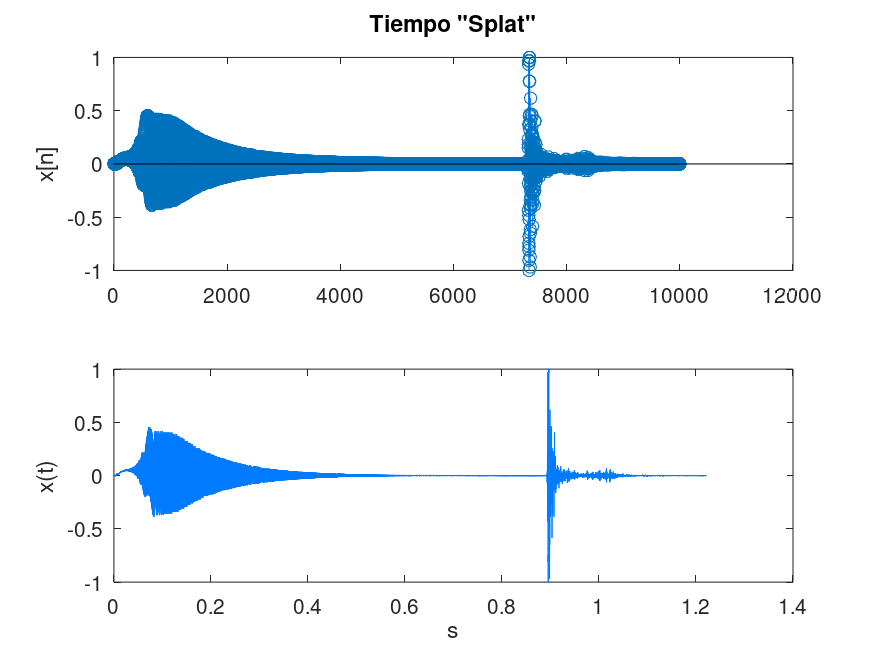
\includegraphics[width=0.7\linewidth]{Imágenes/Figura1}
\end{center}

\begin{lstlisting}
omega = linspace(-3*pi, 3*pi, 3*length(X));
figure(2); subplot(2,1,1);
plot(omega, [abs(X) abs(X) abs(X)], "color", "#007AFF"); xlabel('w'); ylabel('TF (x(t))'); title('T.F dominio continuo de la secuencia');
w = linspace(-length(X)/2, length(X)/2, length(X));
subplot(2, 1,2); plot(w, abs(X), "color", "#007AFF"); xlabel('w'); ylabel('TF (x(t))'); title('T.F dominio continuo');
\end{lstlisting}

\begin{center}
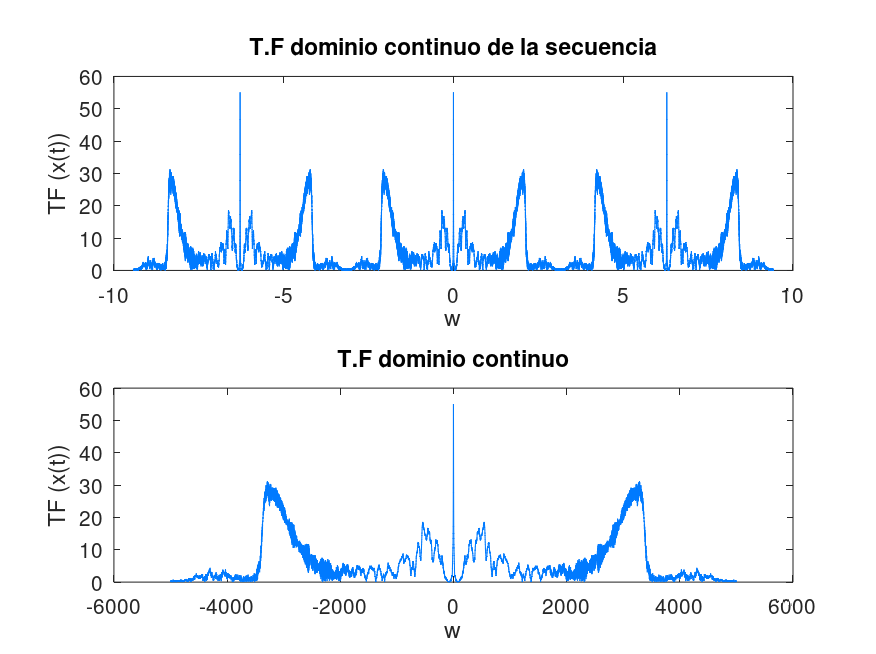
\includegraphics[width=0.7\linewidth]{Imágenes/Figura2}
\end{center}

La interpretación que hacemos de \code{Splat} es la siguiente:
\begin{enumerate}[label=\arabic*)]
	\item Vemos como inicia el sonido con la caída del, por lo tanto vemos el pico de la frecuencia y cómo comienza  a disminuir hasta llegar cercano a cero.
	\item Pasa un cierto periodo de tiempo en el que la frecuencia es cercana a cero hasta que se escucha el impacto del objeto por lo que la frecuencia sube rápidamente hasta 40 y como el sonido del impacto es fuerte pero rápido, una vez sube decrece muy rápidamente.
\end{enumerate}

\item \textbf{Secuencia 'laughter' muestreada a 8 KHz:}
\begin{lstlisting}
load laughter.mat
\end{lstlisting}

\begin{lstlisting}
load laughter.mat
sound(y, Fs);
fs = Fs;
x = y.';
X = ft(x);
n = (1:length(x))/fs;
figure(3); subplot(2,1,1);
stem(x, "color", "#007AFF");title('Tiempo "Laughter"'); ylabel('x[n]');
subplot(2,1,2); plot(n,x,"color", "#007AFF"); xlabel('s'); ylabel('x(t)');
\end{lstlisting}

\begin{center}
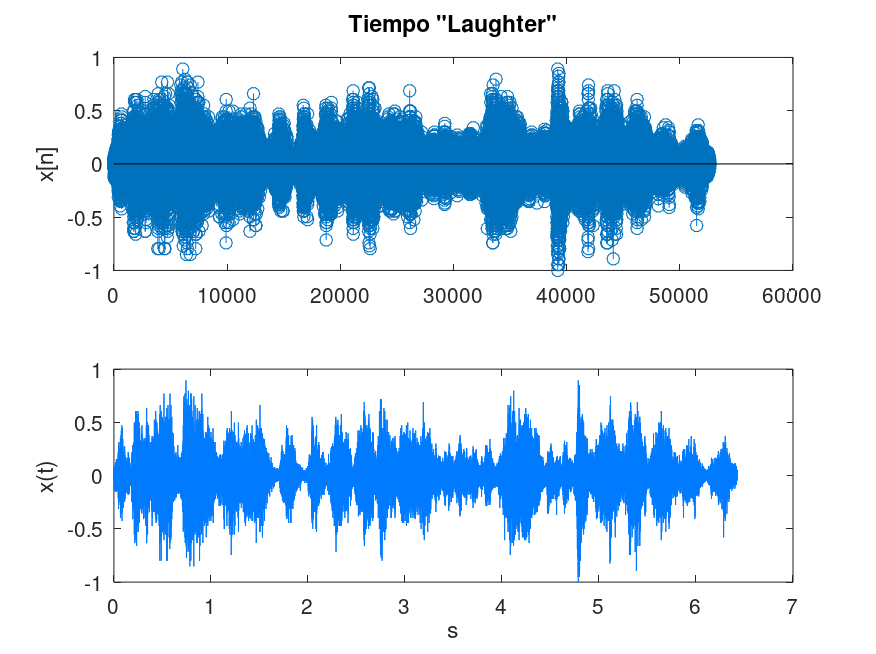
\includegraphics[width=0.7\linewidth]{Imágenes/Figura3}
\end{center}

\begin{lstlisting}
omega = linspace(-3*pi, 3*pi, 3*length(X));
figure(4); title('T.F dominio continuo'); subplot(2, 1,1);
plot(omega, [abs(X) abs(X) abs(X)],"color", "#007AFF"); xlabel('w'); ylabel('TF (x(t))');title('T.F dominio continuo de la secuencia');
w = linspace(-length(X)/2, length(X)/2, length(X));
 subplot(2, 1,2); plot(w, abs(X), "color", "#007AFF"); xlabel('w'); ylabel('TF (x(t))'); title('T.F dominio continuo');
\end{lstlisting}

\begin{center}
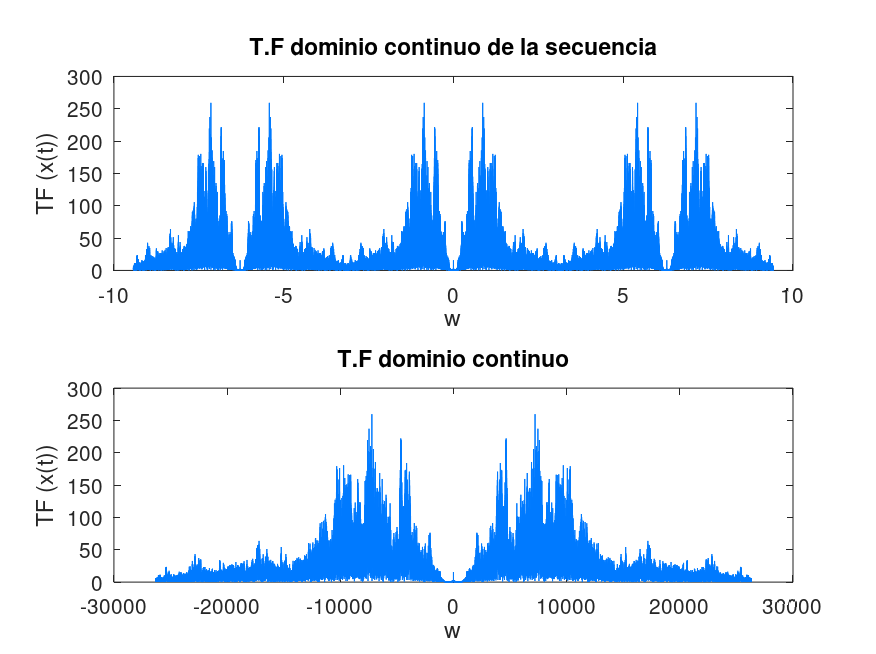
\includegraphics[width=0.7\linewidth]{Imágenes/Figura4}
\end{center}

La interpretación que hacemos de la frecuencia de \code{Laughter} sería la siguiente:
\begin{enumerate}[label=\arabic*)]
	\item Podemos observar cómo crece rápidamente la frecuencia con el inicio de las carcajadas de la multitud y se producen tres variaciones de bajada y subida que coinciden con el espacio de sonido vacío entre unas carcajadas y otras.
	\item Una vez comienza a disminuirse la cantidad de carcajadas podemos observar cómo la frecuencia disminuye progresivamente, pero no disminuye de forma drástica desde un pico de frecuencia hasta cero tal como ocurría con la frecuencia anterior.
\end{enumerate}

\item \textbf{Secuencia 'handel' muestreada a 8 KHz:}
\begin{lstlisting}
load handel.mat
\end{lstlisting}

\begin{lstlisting}
load handel.mat
sound(y, Fs);
fs = Fs;
x = y.';
X = ft(x);
n = (1:length(x))/fs;
figure(5);subplot(2,1,1);
stem(x);title('Tiempo "Handel"'); ylabel('x[n]');
subplot(2,1,2);
plot(n,x,"color", "#007AFF"); xlabel('s'); ylabel('x(t)');
\end{lstlisting}

\begin{center}
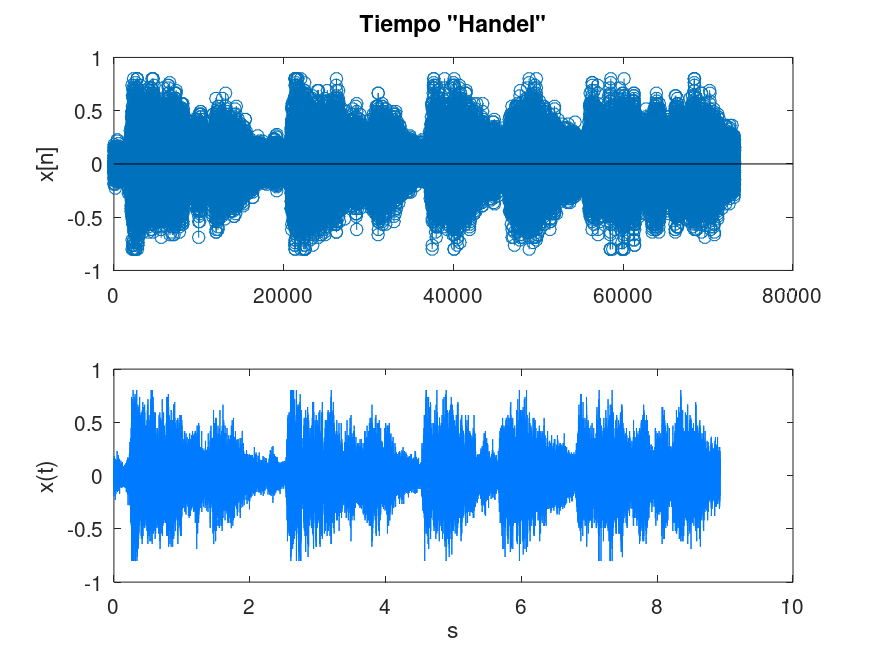
\includegraphics[width=0.7\linewidth]{Imágenes/Figura5}
\end{center}

\begin{lstlisting}
omega = linspace(-3*pi, 3*pi, 3*length(X));
figure(6); title('T.F dominio continuo'); subplot(2, 1,1);
plot(omega, [abs(X) abs(X) abs(X)], "color", "#007AFF"); xlabel('w'); ylabel('TF (x(t))');title('T.F dominio continuo de la secuencia');
w = linspace(-length(X)/2, length(X)/2, length(X));
 subplot(2, 1,2); plot(w, abs(X), "color", "#007AFF"); xlabel('w'); ylabel('TF (x(t))');title('T.F dominio continuo');
\end{lstlisting}

\begin{center}
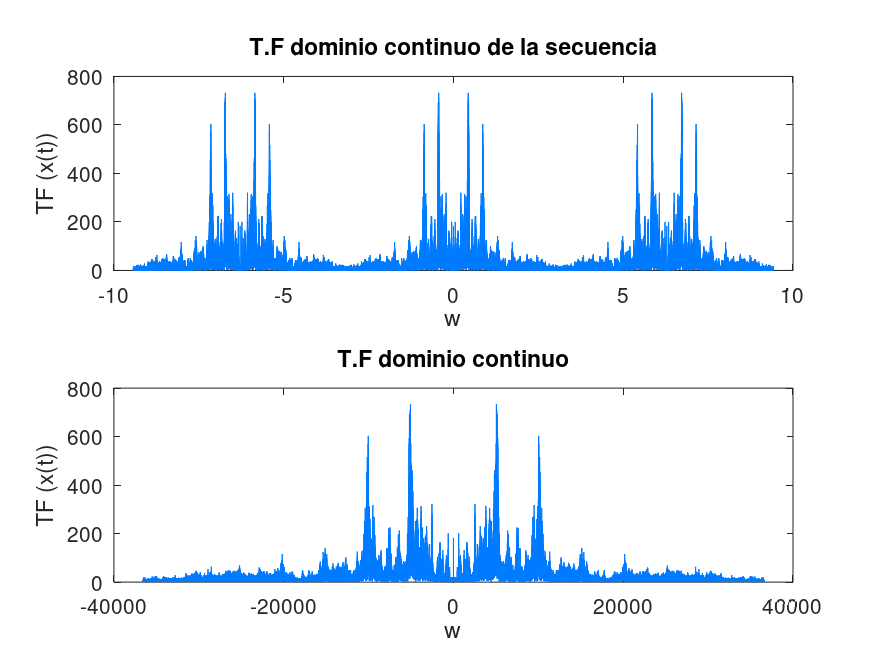
\includegraphics[width=0.7\linewidth]{Imágenes/Figura6}
\end{center}

La frecuencia corresponde al final de la ópera \textbf{El Mesías} de Haendel, \textit{Aleluya}. En la interpretación se escuchan cinco \textit{Aleluya}s donde en cuatro de ellos se produce un pico debido a la entonación del principio de estrofa (\textbf{\textit{"A"}}), podemos observar una frecuencia similar que se va repitiendo a excepción del quinto donde la entonación cambio totalmente para marcar el final de frase, por lo que en la última estrofa se observa la reducción de frecuencia con respecto a las otras.

\end{itemize}
\section{Comparativa del coste computacional DFT y FFT}
\subsection*{Cuestiones}
Implemente dos funciones en Matlab:
\begin{itemize}
\item La primera debe emplear la implementación directa con Matlab y su entrada será la secuencia a transformar. La función proporcionará la transformada. Llame a la función \code{mdft.m}
\item La segunda debe implementar la versión eficiente basada en el algoritmo de diezmado en tiempo. El nombre de la función será \code{ffdt.m}
\end{itemize}
Redacte un script en Matlab que obtenga una secuencia real $x$ de longitud $N$ con muestras aleatorias empleando el comando \code{rand}.

Empleando los comandos \code{tic} y \code{toc} establezca el tiempo empleado en calcular su DFT utilizando la función de Matlab \code{mdft.m} y mediante la versión eficaz del mismo denominada \code{ffdt.m}

\begin{lstlisting}
N = 64;

x = rand(1, N);

% Calcular DFT usando mdft.m
tic
X_mdft = mdft(x)
toc

% Calcular DFT usando fftdt.m
tic
X_mdft = fftdt(x)
toc
\end{lstlisting}

Empleando lo siguientes valores para $N=2^{10},2^{11},2^{12},2^{13},2^{14},2^{15},2^{16}$ y $2^{17}$ represente en una misma gráfica los tiempos de cálculo empleados por las dos implementaciones de la DFT respecto al valor de $N$. Etiquete correctamente ambos ejes e incluya la correspondiente leyenda para diferenciar ambas curvas.

\begin{lstlisting}
N_values = 2.^(10:17);

array_mdft = zeros(1, length(N_values));
array_fftdt = zeros(1, length(N_values));

% Calcular DFT y coste computacional
for i = 1:length(N_values)
    x = rand(1, N_values(i));

    tic
    X_mdft = mdft(x);
    array_mdft(i) = toc;

    tic
    X_fftdt = fftdt(x);
    array_fftdt(i) = toc;
end

figure(7); plot(N_values, array_mdft, "color", '#FF0000', "LineWidth", 2, N_values, array_fftdt, "color", '#007AFF', "LineWidth", 2);
xlabel('N'); ylabel('Coste computacional (s)'); legend('DFT', 'FFT')
\end{lstlisting}

\begin{center}
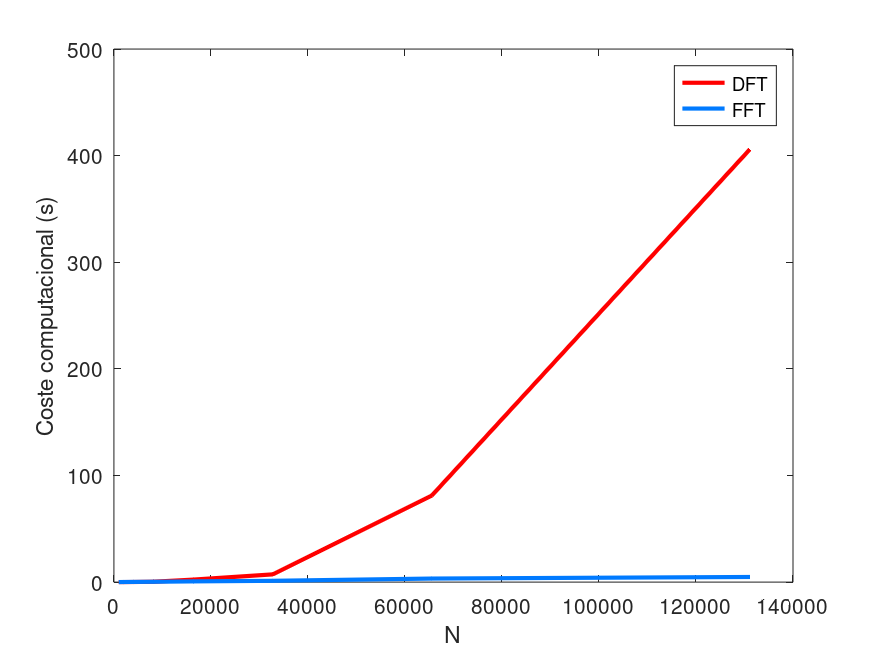
\includegraphics[width=0.7\linewidth]{Imágenes/Figura7}
\end{center}

Podemos observar como la Transformada Rápida de Fourier (FFT) es mucho más eficeiente a nivel de coste computacional que la Transformada Discreta de Fourier (DFT).

\section{Comparativa de convolución lineal vs convolución circular}
\subsection*{Cuestiones}
Implemente el código necesario para generar y representar la convolución lineal de:
\begin{itemize}
\item Una secuencia de números aleatorios de 64 muestras definida en $n=0..63$.
\item Un filtro FIR casual que realice el promedio deslizante de 8 muestras.
\end{itemize}
Utilice la función \code{convcirc(x1,x2,N)} para realizar la convolución circular de $N$ puntos de secuencia y la respuesta al impulso del filtro. Considere el mínimo $N$ posible y represente gráficamente el resultado, etiquetando correctamente el eje temporal, $n=0..N-1$.

Defina la convolución circular de la siguiente manera
\begin{lstlisting}
convcirc = inline('real(ifft(fft(x1, N) .* fft(x2, N), N))', 'x1', 'x2', 'N');
\end{lstlisting}
\begin{itemize}
\item Especifique si proporcionan el mismo resultado la convolución lineal y la convolución circular. Indique las muestras que difieren.
\item Incremente el tamaño $N$ de la convolución circular. Indique el valor de $N$ para el que se obtiene un mismo resultado para ambas convoluciones.
\end{itemize}

\newpage

\begin{lstlisting}
n = 0:63;
x1 = rand(1, 64);

% Filtro FIR
x2 = ones(1, 8) / 8

% Definir la función de convolución circular
convcirc = inline('real(ifft(fft(x1, N) .* fft(x2, N), N))', 'x1', 'x2', 'N');

N = 64;
y_circ = convcirc(x1, x2, N);
y_lineal = conv(x1, x2);

isequal(round(y_circ), round(y_lineal(1:N)))

diff = y_lineal(1:N) - y_circ;
diff

% Aquí podemos observar que los resultados no son iguales, por lo que vamos a
% aumentar el valor de N usando la condición
\end{lstlisting}

\begin{verbatim}
diff =

 Columns 1 through 21:

  -0.4127  -0.3199  -0.2345  -0.1467  -0.1291  -0.0339  -0.0300  -0.0000  -0.0000  -0.0000  -0.0000 
  0.0000   0.0000        0  -0.0000  -0.0000   0.0000   0.0000   0.0000         0   0.0000

 Columns 22 through 42:

   0.0000        0   0.0000        0   0.0000  -0.0000   0.0000   0.0000  -0.0000  -0.0000  -0.0000
  -0.0000        0        0  -0.0000  -0.0000        0        0  -0.0000        0        0

 Columns 43 through 64:

  -0.0000   0.0000        0        0  -0.0000  -0.0000   0.0000        0   0.0000  -0.0000  -0.0000
   0.0000   0.0000  -0.0000  -0.0000        0  -0.0000        0  -0.0000  -0.0000  -0.0000        0
\end{verbatim}

Para que la convolcuión circular y la convolución lineal coincidan se tiene que cumplir la siguiente condición:
\begin{itemize}
\item Que la duración de la señal de salida sea mayor o igual a la suma de las duraciones de las señales menos 1 \linebreak (\code{length(x1) + length(x2) - 1}). 
\end{itemize}
\begin{lstlisting}
N = length(x1) + length(x2) - 1; % N = 71
y_circ = convcirc(x1, x2, N);
y_lineal = conv(x1, x2);

isequal(round(y_circ), round(y_lineal(1:N)))

% Los resultados que nos devuelven son muy parecidos salvo por ciertos errores de redondeo
\end{lstlisting}
\end{document}